% rubber: set program xelatex
\documentclass[a4paper,12pt]{article}

\usepackage{xltxtra}
\usepackage{amsmath,amsthm,amssymb}

\usepackage[autostyle=true]{csquotes}
\usepackage{polyglossia}
\setmainlanguage{english}
\setotherlanguage[variant=mono]{greek}

% Fonts
\setmainfont{CMU Serif}                 
\setsansfont{CMU Sans Serif}            
\setmonofont{CMU Typewriter Text}


\usepackage[margin=1in]{geometry} 

% Source code listings
\usepackage{listings}
\usepackage{color}
\usepackage{matlab-prettifier}
\lstdefinestyle{My-Matlab}
{
  style               = MatlabBaseStyle@mlpr,
  basicstyle          = \color{black}\ttfamily\small,
  mllastelementstyle  = \color{black}                    ,
  mlkeywordstyle      = \color[RGB]{000,000,255}         ,
  mlcommentstyle      = \color[RGB]{034,139,034}         ,
  mlstringstyle       = \color[RGB]{160,032,240}         ,
  mlsyscomstyle       = \color[RGB]{178,140,000}         ,
  mlsectiontitlestyle = \commentStyle@mlpr      \bfseries,
  mlsharedvarstyle    = \color[RGB]{000,163,163}         ,
  mlplaceholderstyle  = \mleditorphstyle,
}
% Disable paragraph intention 
\setlength\parindent{0pt}  


\begin{document}
\title{ Multi-Sensors Fusion and Tracking\\Vibot Program 2018-2019}
\author{Ioannis Tsagatakis\\
1\textsuperscript{st} Assignment: Background Subtraction} 
 
\maketitle

\section{Data Preperation}
To speed up development the image files are read only once and saved as \texttt{'mat'} files. The code for the \texttt{'gtruth.mat'} file is given bellow. The code for the other image sequences is simmilar and it is on the github repository.

\lstinputlisting[style=My-Matlab, firstline=15]{../Data/prepare_data_gtruth.m}

\section{Frame differencing}
The following matlab function implements the \textit{Frame differencing} method.

\lstinputlisting[style=My-Matlab]{../Code/bgsub_frame_diff.m}

To demonstrate we need a fuction to annotate the video with data like frame number and location, and with a bounding box around the main moving object of the scene.

\begin{figure}[Ht]
\centering
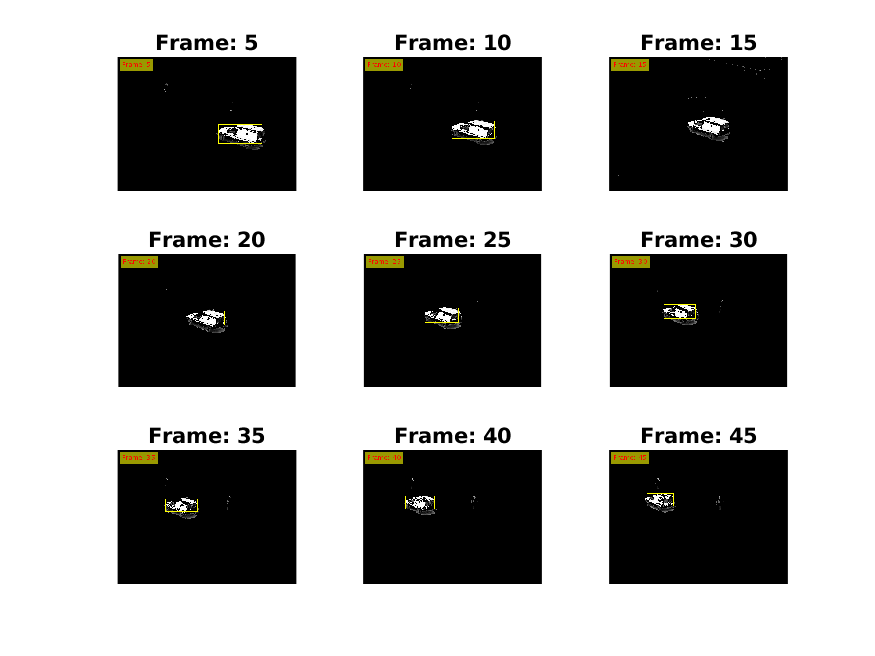
\includegraphics{../Videos/bgsub_framediff_cars.png}
\label{fig:fdiff_cars}
\caption{Frame differencing for the cars sequence}
\end{figure}

\lstinputlisting[style=My-Matlab]{../Code/anotate_video_box.m}

And a code to save the video sequence as a playable video on hard disk.

\lstinputlisting[style=My-Matlab]{../Code/videoSave.m}

Finnaly a fuction is created to save some frames in png file format.
\lstinputlisting[style=My-Matlab]{../Code/video_to_img_seq.m}

\subsection{Cars Sequence}
Let's apply the algorithm to the \texttt{'cars'} sequence.
\lstinputlisting[style=My-Matlab]{../Code/bgsub_demo_cars_fdiff.m}

Some frames is given in Figure~\ref{fig:fdiff_cars} on page \pageref{fig:fdiff_cars}.


\subsection{Highway Sequence}

\begin{figure}[Ht]
\centering
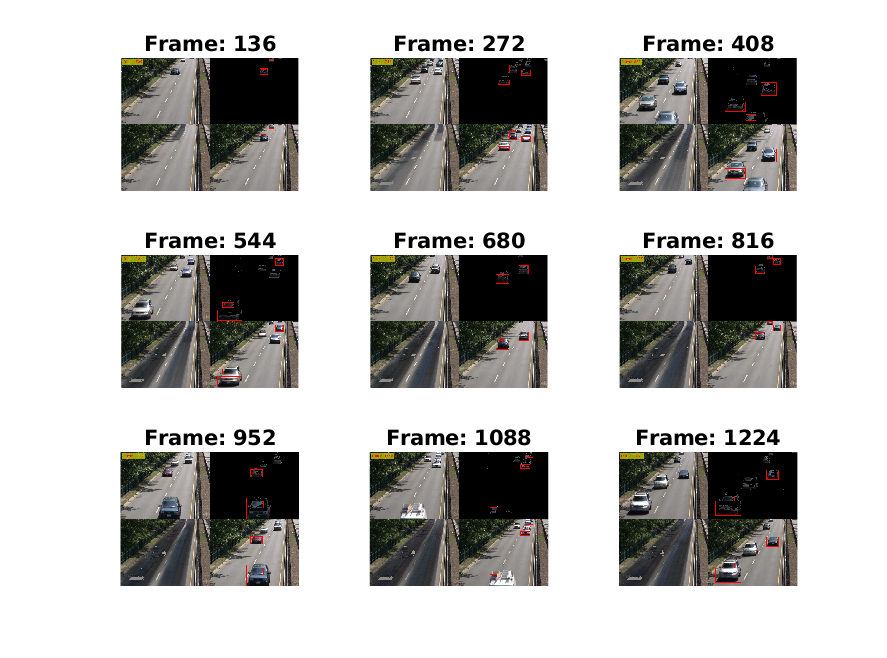
\includegraphics{../Videos/highway_frame_diff.png}
\label{fig:fdiff_highway}
\caption{Frame differencing for the highway sequence}
\end{figure}

The highway sequence is in color. So we modify the algorithm. An Eucledian metric is used  to estimate the threshold of a given pixel form the background. Also the confusion matrix is calculated. After many revisions the final code is given bellow

\vspace{10pt}
\lstinputlisting[style=My-Matlab]{../Code/highway_frame_diff.m}
\vspace{30pt}

Some frames is given in Figure~\ref{fig:fdiff_highway} on page \pageref{fig:fdiff_highway}.

\section{The Running Average Gaussian Method}

\subsection{Cars Sequence}

The code that implements the Running Average Gaussian Method on the cars sequence is given bellow 

\vspace{10pt}
\lstinputlisting[style=My-Matlab]{../Code/a3_gaussian.m}
\vspace{30pt}

Some frames is given in Figure~\ref{fig:a3_gaussian_cars} on page \pageref{fig:a3_gaussian_cars}.
\centering
\begin{figure}[Ht]
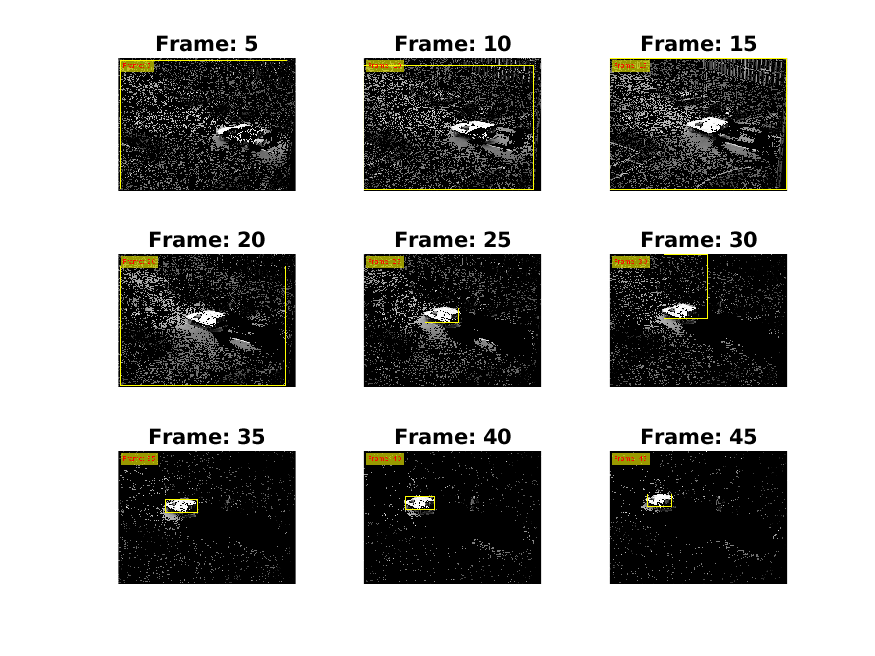
\includegraphics{../Videos/a3_gaussian.png}
\label{fig:a3_gaussian_cars}
\caption{Frame differencing for the highway sequence}
\end{figure}
 

\vfill
\noindent Tools used: \texttt{Matlab}, \LaTeX{}.
\end{document}
